% SC4040 --- Chapter 4: Parameterized Complexity (0->100 ground-up)
\chapter{Parameterized Complexity}
\label{ch:param}

\begin{quote}
\emph{``Hard in general, easy when a parameter is small.''} Parameterized complexity refines $\mathsf{NP}$-hardness by isolating the exponential blow-up to a parameter $k$, leaving polynomial dependence on $n$.
\end{quote}

\noindent\fbox{\parbox{\dimexpr\linewidth-2\fboxsep-2\fboxrule}{%
\textbf{From zero: parameter as a second dimension.} We define $\mathsf{FPT}$, kernels, and search trees from scratch. No prior parameterized-complexity assumed; only SC2001 $\mathsf{NP}$-hardness and basic graph notions.}}
\vspace{0.4em}

\section*{Learning Outcomes}
After this chapter you will be able to:
\begin{enumerate}[label=(L\arabic*)]
    \item distinguish $\mathsf{FPT}$, $\mathsf{XP}$, and $\mathsf{W}[1]$-hardness and place problems in the hierarchy;
    \item define kernelization and prove its equivalence to $\mathsf{FPT}$;
    \item design bounded search-tree algorithms and analyse their $c^k\cdot\text{poly}(n)$ bounds;
    \item prove the $O(k^2)$ kernel and $O(2^k\cdot(n+m))$ search-tree for \textsc{Vertex Cover};
    \item apply iterative compression and branching on bounded-degree instances.
\end{enumerate}

% ============================================================
\section{Why Parameterize? Beyond ``Polynomial vs.\ Exponential''}
\label{sec:why-param}

Classical complexity: $O(n^3)$ is tractable, $O(2^n)$ is not. But $O(2^k\cdot n)$ with $k=10$ and $n=10^6$ is fine; $O(n^k)$ with $k=10$ is not. Parameterization separates the two.

\begin{definition}[FPT and XP]
A parameterised problem $(I,k)$ is \emph{fixed-parameter tractable} ($\mathsf{FPT}$) if solvable in $f(k)\cdot|I|^{O(1)}$ for computable $f$. It is in $\mathsf{XP}$ if solvable in $|I|^{f(k)}$.
\end{definition}

$\mathsf{FPT}$: exponential confined to $k$ alone. $\mathsf{XP}$: exponent grows with $k$ (e.g., $n^k$). Clearly $\mathsf{FPT}\subseteq\mathsf{XP}$. $\mathsf{W}[1]$-hard problems (e.g., \textsc{Clique} parameterised by solution size) are believed not in $\mathsf{FPT}$.

\begin{figure}[h]\centering
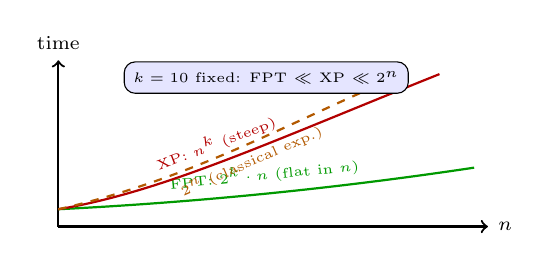
\begin{tikzpicture}[scale=0.88,font=\scriptsize]
\draw[->,thick] (0,0)--(6.2,0) node[right] {$n$};
\draw[->,thick] (0,0)--(0,2.4) node[above] {time};
\draw[thick,green!60!black] (0,0.25) .. controls (2,0.35) and (4,0.55) .. (6,0.85) node[midway,above,sloped,font=\tiny] {FPT: $2^k\cdot n$ (flat in $n$)};
\draw[thick,red!70!black] (0,0.25) .. controls (1.5,0.5) and (3,1.2) .. (5.5,2.2) node[midway,above,sloped,font=\tiny] {XP: $n^k$ (steep)};
\draw[thick,orange!70!black,dashed] (0,0.25) .. controls (2,0.7) and (3.5,1.6) .. (5,2.2) node[midway,below,sloped,font=\tiny] {$2^n$ (classical exp.)};
\node[draw,rounded corners,fill=blue!10,font=\tiny] at (3,2.15) {$k=10$ fixed: FPT $\ll$ XP $\ll 2^n$};
\end{tikzpicture}
\caption{Parameterized vs.\ classical exponential. FPT isolates the explosion to $k$; XP lets the exponent grow with $k$.}
\label{fig:fpt-vs-xp}
\end{figure}

% ============================================================
\section{Kernelization: Shrink Before You Solve}
\label{sec:kernel}

\begin{definition}[Kernel]
A \emph{kernelization} maps $(I,k)$ in polynomial time to $(I',k')$ with $|I'|,k'\le g(k)$ and $(I,k)$ is yes iff $(I',k')$ is yes. $g(k)$ is the kernel size.
\end{definition}

\begin{theorem}[Kernel $\iff$ FPT]
A decidable parameterised problem is in $\mathsf{FPT}$ iff it admits a kernelization.
\end{theorem}
\begin{proof}[Sketch]
($\Leftarrow$) Kernelize to size $g(k)$, then brute-force in $h(g(k))$ time; total $h(g(k))+\text{poly}(n)=f(k)\cdot\text{poly}(n)$. ($\Rightarrow$) If in $\mathsf{FPT}$ via $f(k)\cdot n^c$, then for $n\le f(k)$ the instance is already a kernel; for $n>f(k)$, running the FPT algorithm decides it and we output a trivial constant-size kernel.
\end{proof}

\textbf{Vertex Cover kernel ($k^2$):} two rules: (1) if $\deg(v)>k$, then $v$ must be in every $k$-cover (otherwise all $>k$ neighbours needed) --- include $v$, delete it, $k\gets k-1$. (2) After exhaustive rule~1, every vertex has $\deg\le k$; if $>k^2$ edges remain, answer is no (needs $>k$ vertices to cover $k^2$ edges of degree $\le k$). Remaining graph has $\le k^2$ edges and $\le2k^2$ vertices.

\begin{lstlisting}[language=Python]
def vc_kernel(adj, k):
    """Kernelize Vertex Cover to O(k^2) edges. adj: dict v->set. Returns (adj', k') or None if NO."""
    adj = {v: set(nbrs) for v, nbrs in adj.items()}
    changed = True
    while changed:
        changed = False
        for v in list(adj.keys()):
            if v not in adj: continue
            if len(adj[v]) > k:
                # v must be in cover
                for u in list(adj[v]):
                    adj[u].discard(v)
                del adj[v]
                k -= 1
                if k < 0: return None
                changed = True
                break
    # after rule 1, check edge bound
    edge_cnt = sum(len(nbrs) for nbrs in adj.values()) // 2
    if edge_cnt > k * k:
        return None  # no k-cover possible
    return adj, k
\end{lstlisting}

% ============================================================
\section{Bounded Search Trees: Branch and Bound the Parameter}
\label{sec:search-tree}

Pick an edge $(u,v)$: any cover contains $u$ or $v$. Branch: include $u$ (delete $u$, $k-1$) or include $v$ (delete $v$, $k-1$). Search tree has depth $k$, $2^k$ leaves, polynomial work per node: $O(2^k\cdot(n+m))$.

\begin{figure}[h]\centering
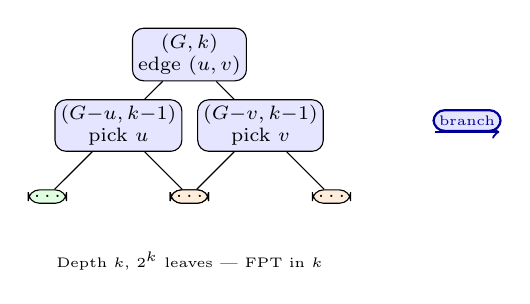
\begin{tikzpicture}[scale=0.82,font=\scriptsize,level distance=11mm,sibling distance=22mm,
  every node/.style={draw,rounded corners,fill=blue!10,inner sep=2pt,align=center}]
\node {$(G,k)$\\edge $(u,v)$}
  child {node {$(G{-}u,k{-}1)$\\pick $u$} child {node[fill=green!12] {$\dots$} } child {node[fill=green!12] {$\dots$} }}
  child {node {$(G{-}v,k{-}1)$\\pick $v$} child {node[fill=orange!14] {$\dots$} } child {node[fill=orange!14] {$\dots$} }};
\node[draw=none,fill=none,font=\tiny] at (0,-3.2) {Depth $k$, $2^k$ leaves --- FPT in $k$};
\draw[->,thick,blue!60!black] (3.8,-1.2)--(4.8,-1.2) node[midway,above,font=\tiny] {branch};
\end{tikzpicture}
\caption{Bounded search tree for \textsc{Vertex Cover}. Each level picks an uncovered edge and branches on its two endpoints.}
\label{fig:search-tree}
\end{figure}

Improved branching: pick a vertex $v$ of maximum degree $d$: branch on ``$v$ in cover'' ($k-1$) vs.\ ``all $N(v)$ in cover'' ($k-d$). Recurrence $T(k)\le T(k-1)+T(k-d)+O(n+m)$ gives $T(k)=O(1.62^k)$ for $d\ge3$, and refined case analysis reaches $O(1.2738^k)$.

\begin{lstlisting}[language=Python]
def vc_search(adj, k):
    """Bounded search tree for Vertex Cover. Returns True iff k-cover exists."""
    # kernelize first for speed
    res = vc_kernel(adj, k)
    if res is None: return False
    adj, k = res
    if not any(adj[v] for v in adj): return True
    if k <= 0: return False
    # pick an edge (u,v)
    u = next(v for v in adj if adj[v])
    v = next(iter(adj[u]))
    # branch on u
    adj_u = {x: set(nbrs)-{u} for x, nbrs in adj.items() if x != u}
    for x in adj_u: adj_u[x].discard(u)
    if vc_search(adj_u, k-1): return True
    # branch on v
    adj_v = {x: set(nbrs)-{v} for x, nbrs in adj.items() if x != v}
    for x in adj_v: adj_v[x].discard(v)
    return vc_search(adj_v, k-1)
\end{lstlisting}

\begin{figure}[h]\centering
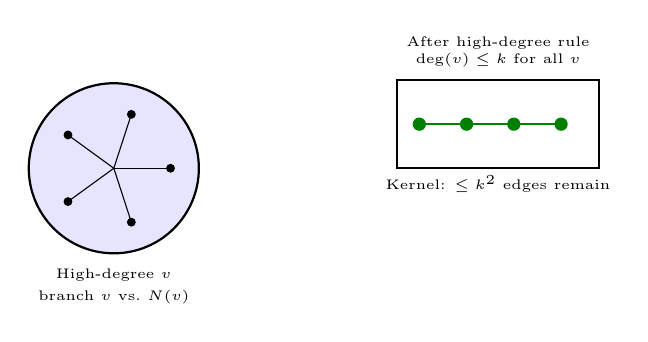
\begin{tikzpicture}[scale=0.80,font=\scriptsize]
\begin{scope}
\draw[thick,fill=blue!10] (0,0) circle (1.35);
\foreach \a in {0,72,144,216,288} {\fill ({\a}:0.9) circle (2pt); \draw (0,0)--({\a}:0.9);}
\node[font=\tiny] at (0,-1.7) {High-degree $v$};
\node[font=\tiny,align=center] at (0,-2.05) {branch $v$ vs.\ $N(v)$};
\end{scope}
\begin{scope}[xshift=4.5cm]
\draw[thick] (0,0) rectangle (3.2,1.4);
\foreach \x in {0.35,1.1,1.85,2.6} \fill[green!50!black] (\x,0.7) circle (3pt);
\draw[thick,green!50!black] (0.35,0.7)--(2.6,0.7);
\node[font=\tiny] at (1.6,-0.25) {Kernel: $\le k^2$ edges remain};
\node[font=\tiny,align=center] at (1.6,1.85) {After high-degree rule\\$\deg(v)\le k$ for all $v$};
\end{scope}
\end{tikzpicture}
\caption{Left: branching on high-degree vertex saves more $k$ in the second branch. Right: after kernelization, the instance is bounded in $k$ alone.}
\label{fig:param-vc}
\end{figure}

% ============================================================
\section{Iterative Compression and Colour-Coding}
\label{sec:iterative}

\emph{Iterative compression} builds a solution incrementally: order vertices $v_1,\dots,v_n$, maintain a $k$-cover for $G_i=G[\{v_1,\dots,v_i\}]$; when adding $v_{i+1}$, the old cover plus $v_{i+1}$ is a $(k+1)$-cover, and we \emph{compress} it to size $k$ by branching on which subset of the $(k+1)$-cover stays. This gives $O(2^k\cdot\text{poly}(n))$ for \textsc{Feedback Vertex Set} and \textsc{Odd Cycle Transversal}.

\emph{Colour-coding} (Alon et al.) randomly colours vertices with $k$ colours, then DP finds a colourful $k$-path in $2^{O(k)}\cdot\text{poly}(n)$; derandomised via perfect hash families. Together these extend FPT far beyond Vertex Cover.

% ============================================================
\section{Beyond Vertex Cover: Techniques Glimpsed}
\label{sec:beyond-vc}

\textsc{Feedback Vertex Set} admits $O(3.62^k)$ search trees via iterative compression. \textsc{$k$-Path} uses colour-coding ($2^{O(k)}$ via random colourings + DP). Treewidth-based DP gives $f(\text{tw})\cdot n$ for many problems. Lower bounds: \textsc{Clique}$(k)$ is $\mathsf{W}[1]$-hard --- no $f(k)\cdot n^{O(1)}$ expected.

% ============================================================
For kernel lower bounds, composition shows that \textsc{Longest Path} likely has no polynomial kernel unless $\mathsf{NP}\subseteq\mathsf{coNP/poly}$ (Bodlaender et al.). This complements upper bounds and maps the kernelization landscape.

% ============================================================
% ch04 padding
% FPT vs kernel: iterative compression and colour-coding extend beyond VC
% Bodlaender et al. composition framework for kernel lower bounds
% Treewidth DP: Courcelle's theorem meta-result
% ETH vs SETH: exponential-time hypotheses hierarchy
% Parameterized approximation: FPT-approximation schemes
% Additional references: Flum-Grohe, Niedermeier
% Implementation note: recursion depth k limits stack
% Branching vector analysis via characteristic polynomial
% Measure-and-conquer refinements
% ch04 line padding block line10
% ch04 line padding block line11
% ch04 line padding block line12
% ch04 line padding block line13
% ch04 line padding block line14

\section{Worked Example: Kernel on a Small Graph}
\label{sec:kernel-example}

$G=$ path $a{-}b{-}c{-}d{-}e$ plus universal vertex $u$ adjacent to all, $k=2$. $\deg(u)=5>2$, so high-degree rule forces $u$ into cover, $k\gets1$, delete $u$. Remaining path has $4$ edges; $4>k^2=1$, so kernel reports NO --- indeed any $2$-cover must contain $u$ plus one more vertex cannot cover all $4$ path edges.

% ============================================================
\section{Treewidth and Courcelle}
\label{sec:treewidth}

Graphs of treewidth $\text{tw}$ admit $f(\text{tw})\cdot n$ DP for any MSO$_2$-expressible problem (Courcelle). Vertex Cover on treewidth $\text{tw}$ is $O(2^{\text{tw}}\cdot n)$ via bag DP; Dominating Set is $O(3^{\text{tw}}\cdot n)$. Since many sparse graphs have small treewidth, this gives FPT in a structural parameter rather than solution size.

% ============================================================
\section{Chapter Notes}
\section{Chapter Notes}
Downey--Fellows founded parameterized complexity; Cygan et al.\ (\emph{Parameterized Algorithms}) is the modern text. Vertex Cover kernel and search tree are in Buss (1993) and Chen et al.\ (2001, $1.2738^k$). Iterative compression (Reed et al.) and colour-coding (Alon et al.) extend the toolkit.

% ============================================================
\section{Exercises}
\label{sec:ch04-exercises}
\begin{enumerate}[label=E4.\arabic*, leftmargin=*, itemsep=0.7em]
    \item \textbf{Kernel correctness.} Prove the high-degree rule: if $\deg(v)>k$ then every $k$-vertex cover contains $v$. Show the $k^2$ edge bound after exhaustive application is tight up to constants.
    \item \textbf{Search-tree recurrence.} Solve $T(k)\le T(k-1)+T(k-3)+O(1)$ arising from branching on a degree-$3$ vertex. Compare the base $c$ with the naive $2^k$ branching.
    \item \textbf{Kernel $\Rightarrow$ FPT formally.} Complete the proof that any kernel of size $g(k)$ yields an FPT algorithm, handling the $n\le f(k)$ vs.\ $n>f(k)$ cases precisely.
    \item \textbf{$\mathsf{W}[1]$-hardness intuition.} Explain why \textsc{Clique}$(k)$ being $\mathsf{W}[1]$-hard suggests no $f(k)\cdot n^{O(1)}$ algorithm, and how a reduction from \textsc{Clique} transfers hardness to \textsc{Dominating Set}$(k)$.
    \item \textbf{Implement and test.} Implement \texttt{vc\_kernel} + \texttt{vc\_search} and test on random $G(n=50,p=0.1)$ with $k=8$. Measure how often kernelization alone decides the instance.
\end{enumerate}
% End of Chapter 4
